Yampa is a Haskell library for functional reactive programming. Functional reactive programming is a high-level declarative style of programming for systems which must respond to continuous streams of input, which are often time dependant, without undue delay. Example of such systems include video games, robots, animations and simulations. Haskell with its lazy evaluation, and separation of pure and impure code doesn't make it obvious how to work in these kinds of domains, without adopting a procedural style, so Yampa was developed to provide a more idiomatic approach.

\section{How does Yampa operate?}

Functional Reactive Programming is about processing signals. At its core, Yampa takes a varying input signal (in applications this might be, for example, the temperature from a temperature sensor), and processes it in some way, providing a corresponding varying output signal on the other side (continuing our imaginary example, this might include information on whether a heater should be on or not). The upper part of Figure \ref{fig:overview} illustrates this idea.

So Yampa is concerned with building objects which can take a continuously varying input and provide a corresponding continuously varying output. If we refer to values which continuously vary as \emph{signals}, then Yampa is a library concerned with building and using \emph{signal functions}.

The bulk of Yampa is concerned with building signal functions. However, it is useful to see how a signal function is actually used in real world Haskell code to process signals. The tool that integrates signal functions into normal Haskell code is called \hask{reactimate}. \hask{reactimate} is a sample-process-output loop. The bottom part of Figure \ref{fig:overview} illustrates an idealised loop. \hask{reactimate} has three important inputs.

First \hask{reactimate} has an input of type \hask{IO a}, whose role is to take a sample of a signal which takes values of type \hask{a}. It might get the position of a mouse cursor, determine whether a key on the keyboard has been pressed, or get the temperature from a temperature sensor. Secondly, \hask{reactimate} needs a signal function, which is described using Yampa code. After collecting its input sample, of type \hask{a}, \hask{reactimate} processes it with the signal function and obtains an output sample, of type \hask{b}, say. \hask{reactimate} then has an output action, which knows what to do with this value of type \hask{b} in the outside world. For example, our output sample might be a set of coordinates to position an image on the screen, and our output function will take these coordinates and render the image there. The output \hask{IO} action comes back with a value of type \hask{Bool}, which encodes whether reactimate should continue looping or stop. So the input to \hask{reactimate} which describes how our signal should be output to the word is of type \hask{b -> IO Bool}.

Clearly, \hask{reactimate} should be capable of input and output, and so it should be a function in the \hask{IO} monad, and indeed, \hask{reactimate} returns a value of type \hask{IO ()}. In addition, \hask{reactimate} should receive some initialisation information, again of type \hask{IO a}.

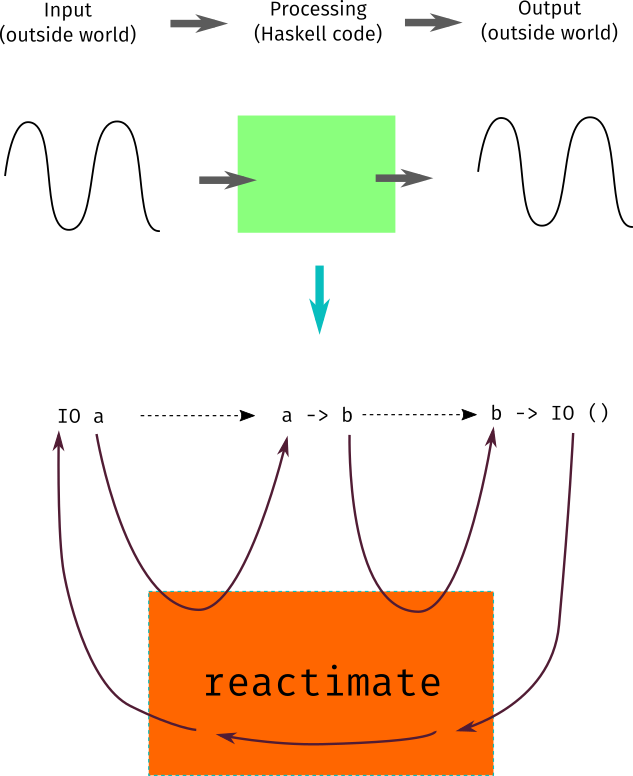
\includegraphics[height=300pt]{Diagrams/overview.png}

So \hask{reactimate} continuously samples the input, processes it with a signal function, and performs some output, until our output function says to stop. The above captures the essence of what reactimate does, but in reality the type of reactimate is a little more opaque:

\begin{lstlisting}
reactimate :: IO a
    -> (Bool -> IO (DTime, Maybe a))
    -> (Bool -> b -> IO Bool)
    -> SF a b
    -> IO ()
\end{lstlisting}

The first \hask{IO a} here is the initialisation input, and the value of type \hask{a} is the value of the first sample. The second input, of type \hask{Bool -> IO (DTime, Maybe a)} is our input function. In the definition of \hask{reactimate} the input value of \hask{Bool} is unused, so really one just needs to specify a value of type \hask{IO (DTime, Maybe a)}. In fact to make this simpler, lets define

\begin{lstlisting}
sInput :: IO (DTime, Maybe a) -> Bool -> IO (DTime, Maybe a)
sInput inp _ = inp
\end{lstlisting}

\noindent to convert a value of type \hask{IO (DTime, Maybe a)} in a value of type \hask{Bool -> IO (DTime, Maybe a)}. Now lets examine the values wrapped in the \hask{IO} type. First \hask{DTime}: \hask{reactimate} doesn't have a built in time tracking system, so on each sample of the input signal, one is required to input the elapsed time since the last sample was taken. \hask{DTime} is a synonym for \hask{Double} used to represent this. Later, we define our own reactimate which should work on any POSIX system, and hides this time tracking. Presumably it is kept visible for systems with less uniform or custom time tracking requirements. The second value here, of type \hask{Maybe a}, is the input sample, wrapped in \hask{Maybe} since there may be no input signal, or our sampling may fail. If a value of \hask{Nothing} is fed in, then the value from the previous sample is used.

The third input to \hask{reactimate} specifies how to deal with output. Again, the first \hask{Bool} in \hask{(Bool -> b -> IO Bool)} is unused, so lets define

\begin{lstlisting}
sOutput :: (b -> IO Bool) -> Bool -> b -> IO Bool
sOutput out _ = out
\end{lstlisting}

\noindent to wrap a value of type \hask{b -> IO Bool} in the type required for \hask{reactimate}. The value of type \hask{b -> IO Bool} works as described above, where a value of \hask{True} from the output function indicates to \hask{reactimate} that it should stop. The fourth value of type \hask{SF a b} is the signal function, processing a signal taking values of type \hask{a} into a signal taking values of type \hask{b}. Yampa is concerned with building these signal functions. This will be the subject of (most of) the remainder of this guide.

Using our simplified input and output wrappers, we define a simplified version of \hask{reactimate}:

\begin{lstlisting}
sReactimate :: IO a -> IO (DTime, Maybe a) -> (b -> IO Bool) -> SF a b -> IO ()
sReactimate init inp out sigFun = reactimate init (sInput inp) (sOutput out) sigFun
\end{lstlisting}

\noindent which looks a little clearer, and more like what we discussed above. In fact, we will define a function \yampaMain

\begin{lstlisting}
yampaMain :: IO a -> IO (Maybe a) -> (b -> IO Bool) -> SF a b -> IO ()
\end{lstlisting}

\noindent which also deals with the timing in POSIX compatible systems. We write this in a module \hask{YampaUtils.hs} which we will use in the rest of this guide. Listing \ref{lst:yampaUtils} gives the complete contents of the module. Note \yampaMain is essentially the same as \hask{sReactimate} but wrapped in a time tracking system.

\lstinputlisting[caption={YampaUtils.hs}, frame=single, label=lst:yampaUtils]{./src/YampaUtils.hs}

\section{The structure of a Yampa program}

One can think of Yampa programs as programs of the form illustrated in Listing \ref{lst:generalForm}. To write a Yampa program, we need to specify an initialization, input and an output function, and also construct a signal function to do the required transformations. We then feed all this in to \yampaMain which does the processing we require.

\begin{lstlisting}[caption={General form of a Yampa program}, label={lst:generalForm}]
import FRP.Yampa as Y
import YampaUtils

init :: IO a
-- Do some initialisation

input :: IO (Maybe a)
-- Get some input

output :: b -> IO Bool
-- Do some output

sigFun :: SF a b
-- Do some signal transformations

main :: IO ()
main = yampaMain init input output sigFun
\end{lstlisting}

Of course, real programs will take many different forms, but the idealised above form illustrates what we need to build in order to have an executable program.

\section{Signals and signal functions}

Yampa is a library for building and using signal functions. We have deliberately avoided making precise what is meant by a signal for two reasons

One can think of a signal taking values of type \hask{a}, or more succintly a signal of type \hask{a}, as a value of type \hask{a} with a context. Indeed, one can really think of it as being a value of type \hask{IO a} (see for instance \hask{getPOSIXTime} and compare it with the output from the \hask{time} signal function later). Like any other value of type \hask{IO a}, extracting values at different times can yield different results.
